\chapter{بيولوجيا الصون}\label{ch:b3:conservation-biology}

في عام 1813 راقب أودوبون سربًا من الحمام الزاجر يعبر فوق
كنتاكي ثلاثة أيام، فيُظلم السماء؛ ولعلها كانت خمسة
مليارات، أي ربع طيور أمريكا الشمالية كلها. وفي
1~أيلول 1914 ماتت آخر واحدة، وهي أنثى تُسمّى مارثا، في حديقة
سنسيناتي. ولم يكن النوع نادرًا حين بدأ تراجعه؛ بل
كان يُحصد بأحمال القطارات، وتُقطع غاباته، وطائر
لم يكن يتكاثر إلا في مستعمرات هائلة لم يقدر على التكاثر متى
رقّت المستعمرات دون حجم لم يقسه أحد. وفي عام 1995 كان الكاكابو،
وهو ببغاء ليلي عديم الطيران في نيوزيلندا، قد هبط إلى واحد
وخمسين طائرًا؛ وقد سُمّي كل واحد منها منذ ذلك الحين ووُزن
وزُوّد بمرسل، وقُدّمت له في اللحظة الصحيحة وجبة تكميلية،
وصارت مئتين وخمسين. وفي السنة نفسها أُطلق واحد وثلاثون ذئبًا
رماديًا في يلوستون، بعد سبعين سنة من قتل آخر قطيع
أصلي؛ وفي غضون عقدين انتقلت الأيائل، وعادت
شجيرات الصفصاف على امتداد الأنهار، وعادت معها القنادس.
وبيولوجيا الصون تطبيقُ وراثة الجمهرات وإيكولوجيتها وسلوكها
في هذا الكتاب على سؤال عملي واحد --- كيف
تُمنع الأنواع من الزوال --- وحسابها هو حساب الأعداد الصغيرة.

\section{لماذا تموت الجمهرات الصغيرة}

\begin{definition}[مخاطر الصغر]\label{def:b3:conservation-biology:small}
\index{عشوائية ديموغرافية}\index{عشوائية بيئية}\index{أثر ألي}\index{دوامة الانقراض}\index{أدنى جمهرة قابلة للبقاء}
تتراجع الجمهرة الكبيرة حين يتجاوز معدل وفاتها معدل مواليدها؛
وأما الصغيرة فتقدر على الزوال بلا أي تغيّر في أيهما.
و\emph{العشوائية الديموغرافية} هي حظ أن يموت، بين بضعة
أفراد، أكثر مما يولد، أو أن يكون الناجون كلهم
ذكورًا: وهي تهم دون بضع عشرات. و\emph{العشوائية البيئية}
--- شتاء سيئ، أو جفاف، أو مرض --- تضرب كل فرد دفعةً
واحدة، وجمهرة من بضع مئات كانت الكبيرة ستجتازها
يمكن أن تُمحى؛ و\emph{الكوارث} ذيلها. و\emph{أثر
ألي} يجعل معدل النمو للفرد يهبط عند الكثافة المنخفضة ---
إذ لا تُوجد الأزواج، ولا تقدر المتكاثرات المستعمِرة على
التعشيش، ولا تقدر القطعان على الدفاع عن صغارها، ولم تقدر
أسراب الحمام الزاجر على إشباع المفترسات التي كانت تأخذ فراخه
--- فتتراجع الجمهرة نحو الصفر من تلقاء نفسها دون كثافة عتبية.
ودون بضع مئات، تخفض العمليات الوراثية في القسم التالي
الملاءمةَ جيلًا بعد جيل. وهذه تغذي بعضها بعضًا: فالجمهرة
الأصغر تفقد تباينًا، وتصير أقل خصوبة، وتصغر أكثر، ويزداد
احتمال أن تصيبها المصادفة، فتفقد أكثر --- وتلك \emph{دوامة
الانقراض} (غيلبن وسولي، 1986). و\emph{أدنى جمهرة قابلة للبقاء}
هي الحجم الذي يكون فوقه احتمال الانقراض على أفق معلن
(ولنقل \qty{5}{\%} في قرن) مقبولًا؛ وهو يتوقف على بيولوجيا
النوع وعلى مقدار تقلب بيئته، وهو عادةً بالآلاف.
\end{definition}

\begin{omfigure}
\begin{tikzpicture}[every node/.style={font=\scriptsize}, >=stealth]
  \node[draw, thick, rounded corners, fill=omThm!20, align=center] (small) at (0,0) {الجمهرة\\تصير صغيرة};
  \node[draw, thick, rounded corners, fill=omDef!20, align=center] (drift) at (3.4,1.6) {انجراف وتزاوج داخلي:\\يُفقد التباين، ويرتفع $F$};
  \node[draw, thick, rounded corners, fill=omDef!20, align=center] (fit) at (6.8,0) {تهبط الملاءمة:\\صغار أقل، ومرض أكثر};
  \node[draw, thick, rounded corners, fill=omDef!20, align=center] (chance) at (3.4,-1.6) {المصادفة الديموغرافية والبيئية\\تعضّ أشد};
  \node[draw, thick, rounded corners, fill=omProp!25, align=center] (allee) at (9.9,0) {أثر ألي:\\معدل النمو سالب};
  \draw[->, very thick] (small) -- (drift); \draw[->, very thick] (drift) -- (fit); \draw[->, very thick] (fit) -- (chance); \draw[->, very thick] (chance) -- (small);
  \draw[->, thick, omProp!80!black] (fit) -- (allee); \draw[->, thick, omProp!80!black] (allee.south) .. controls (9.9,-3) and (0,-3.4) .. (small.south);
  \node[align=center, font=\tiny] at (3.4,0) {دوامة الانقراض:\\كل دورة تقلّص\\الجمهرة وتسرّع التالية};
  \node[left, align=right, font=\tiny] at (-1.7,1.5) {فقد الموئل، والحصاد،\\والمفترسات الغازية، والمرض\\تدفع الجمهرة إلى الداخل};
  \draw[->, thick, gray] (-1.6,1.2) -- (small.north west);
\end{tikzpicture}

{\small \omterm{def:b3:conservation-biology:small}{دوامة الانقراض}. ضربة خارجية تجعل الجمهرة
صغيرة؛ ثم يفقد الصغرُ التباينَ، ويخفض الملاءمة، ويعرّض
الجمهرة للمصادفة، ويجعلها أصغر بعد. ومهمة الصون
أن يكسر العروة قبل أن تنغلق.}
\end{omfigure}

\begin{theorem}[الحجم الفعال للجمهرة]\label{thm:b3:conservation-biology:ne}
\index{حجم فعال للجمهرة}\index{نسبة الجنسين}\index{وسط توافقي}\index{معامل التزاوج الداخلي}\index{تغايرية زيجية}
المعدل الذي تفقد به الجمهرة تباينها وتراكم به التزاوج
الداخلي لا يحكمه حجم تعدادها $N$ بل
\emph{حجمها الفعال} $N_{e}$: أي حجم جمهرة مثالية ---
ثابتة، متزاوجة عشوائيًا، متساوية \omterm{thm:b3:conservation-biology:ne}{نسبة الجنسين}، بأحجام أسر
بواسونية --- تفقد \omterm{thm:b3:conservation-biology:ne}{التغايرية الزيجية} بالمعدل نفسه. وثلاثة
انحرافات عن المثالية تخفضه. فأولها نسبة جنسين غير متساوية، عند
$N_{m}$ ذكرًا متكاثرًا و$N_{f}$ أنثى:
\[
N_{e} = \frac{4N_{m}N_{f}}{N_{m} + N_{f}} ;
\]
فذكر واحد ومئة أنثى يعطون $N_{e} \approx 4$. وثانيها تقلب الحجم
على مدى $t$ جيل: فيكون $N_{e}$ هو \emph{\omterm{thm:b3:conservation-biology:ne}{الوسط التوافقي}} لأحجام
الأجيال، $1/N_{e} = (1/t)\sum 1/N_{i}$، يهيمن عليه
الأصغر --- فجمهرة من ألف مرّت مرة بعشرة
يكون $N_{e}$ عندها قرب مئة على ذلك المدى. وثالثها أن تباين حجم الأسرة
فوق البواسوني يخفضه أكثر. وفي جمهرة حجمها الفعال
$N_{e}$ يرتفع \emph{\omterm{thm:b3:conservation-biology:ne}{معامل التزاوج الداخلي}} $F$ --- أي احتمال
أن يكون الأليلان عند موضع في فرد نسختين من أليل سلفي
واحد --- بمقدار $1/2N_{e}$ في الجيل،
\[
F_{t} = 1 - \Bigl(1 - \frac{1}{2N_{e}}\Bigr)^{t} \approx \frac{t}{2N_{e}},
\qquad H_{t} = H_{0}\Bigl(1 - \frac{1}{2N_{e}}\Bigr)^{t} ,
\]
وتخمد \emph{\omterm{thm:b3:conservation-biology:ne}{التغايرية الزيجية}} $H$ بالمعدل نفسه. وقاعدة
فرانكلين الإبهامية، ``50/500'': أما $N_{e} \ge 50$ فيبقي التزاوج الداخلي
دون \qty{1}{\%} في الجيل، وهو المعدل الذي يحتمله مربّو الحيوان؛
و$N_{e} \ge
500$ يدع الطفر يحل محل التباين الذي يزيله الانجراف. ولأن $N_{e}$
عادةً عُشر حجم التعداد، تطلب القاعدة جمهرات
من خمسمئة إلى خمسة آلاف.
\end{theorem}
\begin{proof}
عروسان تُسحبان عشوائيًا من الجمهرة تكونان نسختين من الأليل
الوالدي نفسه باحتمال $1/2N$ في الجمهرة المثالية، وهو
زيادة $F$؛ \omterm{thm:b3:conservation-biology:ne}{والتغايرية الزيجية} $1 - F$ مدرَّجًا، فيضربها كل
جيل في $(1 - 1/2N_{e})$، فينتج الخمود
الأسّي، وينتج، عند $t \ll N_{e}$، الارتفاع الخطي في $F$. وأما \omterm{thm:b3:conservation-biology:ne}{نسبة الجنسين}:
فنصف المورّثات يأتي من كل جنس، فيكون حظ أن تتشارك
عروسان أليلًا والديًا $\tfrac{1}{4}\cdot\tfrac{1}{2N_{m}} +
\tfrac{1}{4}\cdot\tfrac{1}{2N_{f}}$ (إذ يكون ربع الأزواج
أبويين، وربعها أمويين)؛ وبمساواة ذلك بالمقدار $1/2N_{e}$
نجد $1/N_{e} = 1/(4N_{m}) + 1/(4N_{f})$، وهي الصيغة. وأما التقلب:
\omterm{thm:b3:conservation-biology:ne}{فالتغايرية الزيجية} بعد $t$ جيل هي $H_{0}\prod(1 - 1/2N_{i})
\approx H_{0}\exp(-\sum 1/2N_{i})$، وهي تساوي $H_{0}\exp(-t/2N_{e})$
حين يكون $1/N_{e}$ وسطي المقادير $1/N_{i}$. والتزاوج الداخلي يخفض
الملاءمة لأنه يكشف الأليلات المتنحية الضارة
متماثلةَ الزيجة --- وهو \emph{تدهور التزاوج الداخلي}، أي هبوط بضع في المئة
في البقاء أو الخصوبة لكل \qty{10}{\%} من $F$ في معظم الأنواع
المتغايرة التزاوج.
\end{proof}

\begin{omfigure}
\begin{tikzpicture}
\begin{axis}[
  width=0.46\linewidth, height=5.2cm,
  axis x line=bottom, axis y line=left,
  xmin=0, xmax=1, ymin=0, ymax=1.05,
  xlabel={نسبة المتكاثرين الذكور}, ylabel={$N_{e}/N$},
  xlabel style={font=\small, at={(axis description cs:0.5,-0.12)}, anchor=north}, ylabel style={font=\small},
  tick label style={font=\small}, xtick={0,0.1,0.5,0.9,1}, ytick={0.36,1},
  clip=false,
]
\addplot[very thick, omDef, domain=0.005:0.995, samples=100] {4*x*(1-x)};
\draw[dashed, gray] (axis cs:0.1,0) -- (axis cs:0.1,0.36) -- (axis cs:0,0.36);
\node[font=\scriptsize, omDef, anchor=south] at (axis cs:0.5,1.0) {تساوي الجنسين: $N_{e} = N$};
\node[font=\scriptsize, anchor=west, align=left] at (axis cs:0.12,0.2) {ذكر واحد من عشرة\\يتكاثر: $N_{e} = 0.36N$};
\end{axis}
\begin{axis}[
  at={(0.5\linewidth,0)}, anchor=south west,
  width=0.46\linewidth, height=5.2cm,
  axis x line=bottom, axis y line=left,
  xmin=0, xmax=100, ymin=0, ymax=1.05,
  xlabel={الأجيال}, ylabel={التغايرية الزيجية $H_{t}/H_{0}$},
  xlabel style={font=\small, at={(axis description cs:0.5,-0.12)}, anchor=north}, ylabel style={font=\small},
  tick label style={font=\small}, xtick={0,25,50,75,100}, ytick={0.37,0.6,0.9,1},
  yticklabels={0.37,0.6,0.9,1},
  clip=false,
]
\addplot[very thick, omThm, domain=0:100, samples=60] {(1-1/20)^x};
\addplot[very thick, omMeth!70!black, domain=0:100, samples=60] {(1-1/100)^x};
\addplot[very thick, omDef, domain=0:100, samples=60] {(1-1/1000)^x};
\node[font=\scriptsize, omThm, anchor=north west] at (axis cs:12,0.55) {$N_{e} = 10$};
\node[font=\scriptsize, omMeth!70!black, anchor=south west] at (axis cs:50,0.62) {$N_{e} = 50$};
\node[font=\scriptsize, omDef, anchor=south west] at (axis cs:60,0.95) {$N_{e} = 500$};
\end{axis}
\end{tikzpicture}

{\small يسارًا: كيف يقلّص انحراف \omterm{thm:b3:conservation-biology:ne}{نسبة الجنسين} الحجمَ الفعال ---
فنوع الحريم الذي يتكاثر عُشر ذكوره يكون $N_{e}$ عنده ثلث
تعداده. ويمينًا: \omterm{thm:b3:conservation-biology:ne}{التغايرية الزيجية} تخمد بمقدار $(1 - 1/2N_{e})$ في
الجيل --- فجمهرة من عشرة تفقد معظم تباينها في
قرن، وجمهرة من خمسمئة لا تكاد تفقد شيئًا.}
\end{omfigure}

\begin{proof}[شواهد]
الفهد الفلوريدي، وقد هبط إلى نحو خمسة وعشرين حيوانًا في
التسعينيات، أظهر ذيولًا معقوفة وخصًى غير نازلة وعيوبًا قلبية ونطافًا
كان \qty{90}{\%} منها شاذًا --- أي تدهور تزاوج داخلي مرئي؛
وثماني إناث أُدخلت من تكساس عام 1995 (\emph{إنقاذ وراثي})
ثلّثت الجمهرة وتراجعت العيوب. وذئاب جزيرة
رويال، التي أسسها زوج عام 1949 وعُزلت، تراجعت إلى فردين
شديدي التزاوج الداخلي بحلول 2018 مع تشوهات شوكية في معظم
الهياكل المفحوصة. ودجاجة البراري الكبرى في إلينوي هبطت من
آلاف إلى خمسين، وهبط معدل فقس بيضها من \qty{93}{\%} إلى
\qty{56}{\%}، فتعافى بعد أن جُلبت طيور من ولايات أخرى.
وقد أتاحت جلود المتاحف وDNA القديم قياس فقد \omterm{thm:b3:conservation-biology:ne}{التغايرية
الزيجية} مباشرةً في مقابل الجمهرة السابقة للتراجع في كل حالة.
\end{proof}

\begin{omfigure}
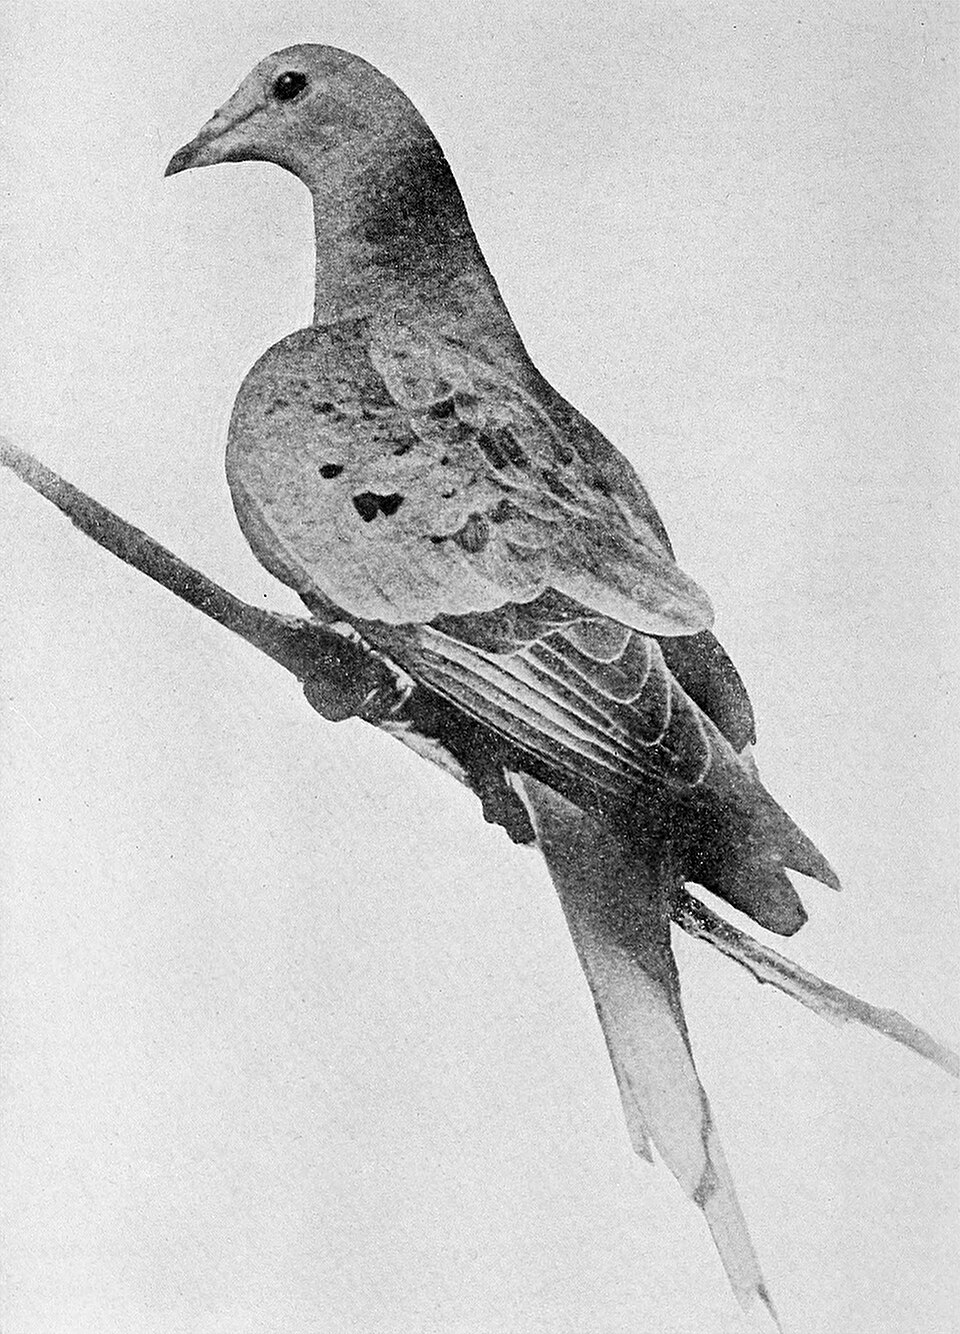
\includegraphics[width=0.4\linewidth]{images/book5/martha.jpg}\hspace{0.04\linewidth}
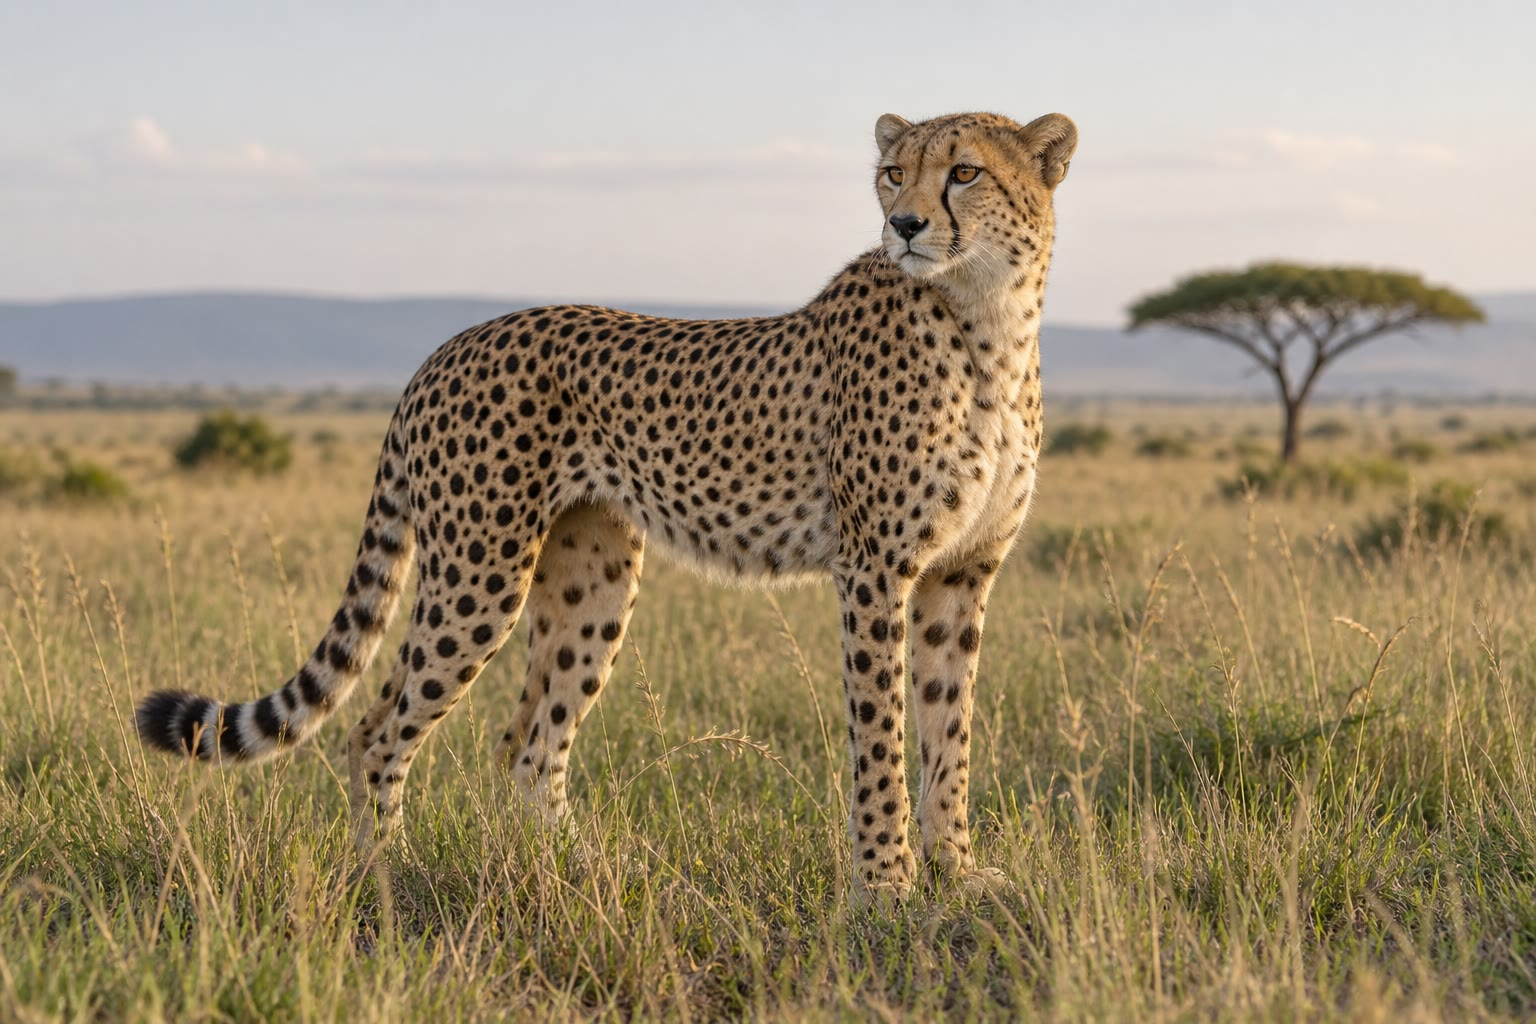
\includegraphics[width=0.52\linewidth]{images/book5/ai/b5-27-cheetah.jpg}

{\small يسارًا: مارثا، آخر حمامة زاجرة، مصوَّرةً في
حديقة سنسيناتي عام 1912؛ وقد كان النوع بالمليارات في حدود
ذاكرة الأحياء (صورة بعدسة إنو ماير، ملكية عامة). ويمينًا:
فهد صياد --- وهو نوع مرّ بعنق زجاجة قبل نحو عشرة آلاف
سنة وأفراده متشابهون حتى إن طعوم الجلد بين
حيوانات غير قريبة لا تُرفض.}
\end{omfigure}

\section{الموئل: كم، وبأي شكل}

\begin{proposition}[الأنواع والمساحة]\label{prop:b3:conservation-biology:area}
\index{علاقة الأنواع بالمساحة}\index{تفتيت الموئل}\index{جغرافيا حيوية للجزر}\index{ممر}\index{جدل SLOSS}\index{أثر الحافة}
عبر الجزر، وعبر شظايا الموائل التي تسلك سلوك الجزر،
يرتفع عدد الأنواع $S$ مع المساحة $A$ بقانون أسّي،
\[
S = c\,A^{z}, \qquad z \approx 0.15\text{--}0.35,
\]
وهي \emph{\omterm{prop:b3:conservation-biology:area}{علاقة الأنواع بالمساحة}} (أرينيوس، 1921؛ وفسّرتها
\omterm{prop:b3:conservation-biology:area}{الجغرافيا الحيوية للجزر} عند مكارثر وويلسون، 1967، ميزانًا بين
الهجرة والانقراض، والانقراض أسرع في الجزر الصغيرة).
فعند $z = 0.25$، يفقد فقدُ \qty{90}{\%} من مساحة موئل في النهاية
$1 - 0.1^{0.25} = \qty{44}{\%}$ من أنواعه؛ ويفقد فقدُ النصف
\qty{16}{\%}. والفقد ليس فوريًا --- بل يُسدَّد \emph{دين انقراض}
على مدى عقود إذ تضمحل جمهرات أصغر من أن تناسب شظاياها
--- ويضيف \emph{تفتيت} مساحة ثابتة إلى قطع فواقد
خاصة به: فكل شظية تحوي جمهرة أصغر، و\emph{آثار الحافة}
(الريح، والحرارة، والمفترسات، والأعشاب) تنفذ مئات الأمتار إلى
داخل الغابة، والأنواع التي تحتاج إلى الداخل تفقد أكثر مما
تفسره المساحة. وأما هل ينقذ محمية واحدة كبيرة أم عدة صغيرة
بالمساحة الكلية نفسها أنواعًا أكثر (وهو \emph{\omterm{prop:b3:conservation-biology:area}{جدل SLOSS}}) فيتوقف
على الأنواع: فالكبيرة تحوي جمهرات أكبر وموئلًا داخليًا،
والصغيرة توزّع خطر كارثة وتعاين
أنماط موائل أكثر. و\emph{الممرات} التي تصل الشظايا تتيح
للأفراد والمورّثات أن تنتقل بينها، فتحيل الجمهرات المعزولة
جمهرةً فوقية يمكن أن يُعاد استعمار أجزائها بعد انقراض
موضعي وأن تُنقذ من التزاوج الداخلي --- ولذلك صارت الأرض
بين المحميات شاغلًا بقدر المحميات نفسها.
\end{proposition}
\begin{proof}
القانون الأسّي تجريبي، مطابق على محورين لوغاريتميين
لأرخبيلات وبحيرات وقمم جبال وشظايا غابات في أنحاء العالم؛ وقيمة
$z$ أدنى لقطع من برّ رئيس (إذ تبقي الهجرةُ الأنواع
حاضرة) وأعلى للجزر الحقيقية. ويتبع الفقد النسبي
مباشرةً: $S'/S = (A'/A)^{z}$. وأما آلية \omterm{prop:b3:conservation-biology:area}{الجغرافيا الحيوية للجزر} فقد
اختبرها سيمبرلوف وويلسون (1969)، إذ بخّرا جزرًا صغيرة من
المانغروف في فلوريدا، فقتلا كل مفصلي، وراقبا أعداد
الأنواع تعود إلى قيمها السابقة في غضون سنة --- أي
توازن، بأنواع غير التي كانت: فالعدد يحدده
المساحة والمسافة، وتحدد الهويات المصادفة.
\end{proof}

\begin{omfigure}
\begin{tikzpicture}
\begin{loglogaxis}[
  width=0.6\linewidth, height=5.4cm,
  axis x line=bottom, axis y line=left,
  xmin=0.5, xmax=20000, ymin=5, ymax=300,
  xlabel={المساحة (km$^2$)}, ylabel={عدد الأنواع},
  xlabel style={font=\small, at={(axis description cs:0.5,-0.12)}, anchor=north}, ylabel style={font=\small},
  tick label style={font=\small}, xtick={1,10,100,1000,10000}, xticklabels={1,10,100,1000,10000}, ytick={10,30,100,300}, yticklabels={10,30,100,300},
  clip=false,
]
\addplot[very thick, omDef, domain=0.5:20000, samples=40] {20*x^0.25};
\addplot[only marks, mark=*, mark size=1.8pt, omDef!70!black] coordinates {(1,22) (3,24) (10,38) (30,44) (100,66) (300,80) (1000,110) (3000,150) (10000,190)};
\draw[dashed, gray] (axis cs:10000,5) -- (axis cs:10000,200) -- (axis cs:0.5,200);
\draw[dashed, gray] (axis cs:1000,5) -- (axis cs:1000,112.5) -- (axis cs:0.5,112.5);
\node[font=\scriptsize, omDef, anchor=south west] at (axis cs:1.2,215) {$S = c\,A^{0.25}$: الميل $z$ على محاور لوغاريتمية};
\node[font=\scriptsize, anchor=west, align=left] at (axis cs:1200,40) {افقد \qty{90}{\%} من المساحة:\\تبقَ على $0.1^{0.25} = \qty{56}{\%}$\\من الأنواع};
\end{loglogaxis}
\end{tikzpicture}

{\small قانون الأنواع والمساحة على محاور لوغاريتمية. وميله
هو الأس $z$؛ ومنه يمكن قراءة الفقد النهائي للأنواع من موئل
متقلّص --- فعُشر الغابة يبقي نحو نصف
الأنواع، لا العُشر الذي كان تخمين خطي سيعطيه.}
\end{omfigure}

\begin{omfigure}
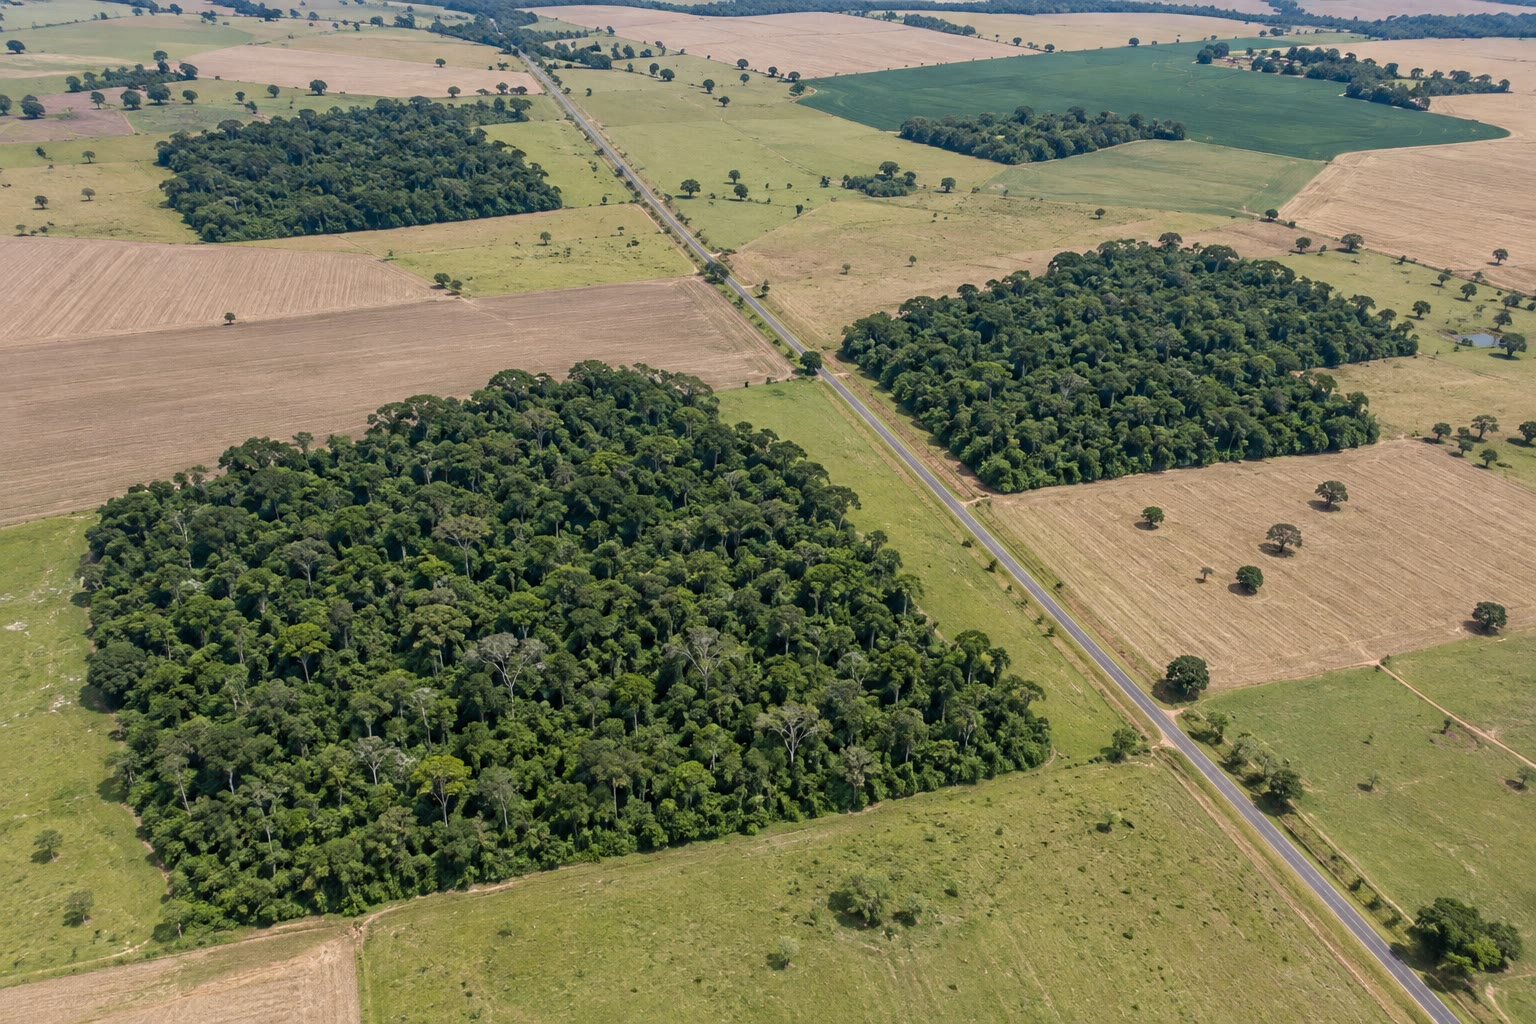
\includegraphics[width=0.6\linewidth]{images/book5/ai/b5-27-forest-fragments.jpg}

{\small شظايا غابة في أرض زراعية، منظورًا إليها من الجو: كل جزيرة
تحوي جمهرة أصغر مما كان الكل يحويه، تحدّها منطقة لا تقدر
أنواع الداخل على استعمالها، ويفصلها حقول لا تقدر أنواع الغابة
على عبورها.}
\end{omfigure}

\section{التنبؤ والوقاية}

\begin{method}[تحليل قابلية الجمهرة للبقاء]\label{met:b3:conservation-biology:pva}
\index{تحليل قابلية الجمهرة للبقاء}\index{شبه انقراض}
لتقدير خطر انقراض جمهرة وما الذي يخفضه:
(1) ابنِ نموذجًا لحركياتها --- مصفوفة من البقاء والخصوبة بحسب
العمر أو الطور، كما في ديموغرافيا مجلد السنة الثانية، مقدَّرة
من أفراد موسومين على مدى عدة سنين؛ (2) وأضف عشوائية ---
ديموغرافية، بسحب مصير كل فرد عشوائيًا،
وبيئية، بسحب معدلات كل سنة من تباينها
المرصود، مع كوارث عرضية؛ (3) وأضف الاعتماد على الكثافة
والتدهور الوراثي للتزاوج الداخلي حيث تسمح البيانات؛ (4) وحاكِ
آلاف المسارات من الحجم الحالي على أفق
الاهتمام وسجّل النسبة التي تهبط دون عتبة \emph{\omterm{met:b3:conservation-biology:pva}{شبه انقراض}}
(أي حجم يُحكم بأن التعافي منه مستحيل)؛ (5) وغيّر
المدخلات --- بقاء البالغين، وبقاء الصغار، ومساحة الموئل،
ونقل عشرة حيوانات --- وانظر أي تغيير يخفض الخطر أكثر؛
فهناك ينبغي أن يذهب الجهد. والمخرج احتمال ذو
ارتياب واسع، لا تنبؤ؛ وقيمته مقارنة، وقد
أظهر مرارًا أن بقاء البالغين، لا الخصوبة، هو الرافعة
في الأنواع الطويلة العمر، ولذلك تقتل خيوطُ الصيد جمهرات
القطرس التي تضع بيضة كل سنتين أسرع من أي فقد
للأعشاش.
\end{method}

\begin{proposition}[زمن الانقراض]\label{prop:b3:conservation-biology:time}
\index{زمن الانقراض}
في جمهرة تتقلب لأن البيئة تتقلب، عند
معدل نمو وسطي $\bar r$ قرب الصفر وتباين $\sigma^{2}$ في
معدل النمو السنوي، يؤدي لوغاريتم حجم الجمهرة مشيًا عشوائيًا
بانسياق، وينمو الزمن المتوقع للانقراض من حجم $N$
مثل \emph{لوغاريتم} $N$ وحده حين $\bar r < 0$ --- فمضاعفة
الجمهرة تضيف عددًا ثابتًا من السنين --- ومثل \emph{قوة} من
$N$ حين $\bar r > 0$، بأس $2\bar r/\sigma^{2} - 1$؛ وتحت
\omterm{def:b3:conservation-biology:small}{العشوائية الديموغرافية} وحدها ينمو \emph{أسيًا} مع
$N$، حتى إن جمهرة آمنة من المصادفة الديموغرافية عند مئة
يمكن أن تُفقد بالتباين البيئي عند عشرة آلاف. والنتيجة
العملية أن خفض تباين نمو جمهرة --- بحمايتها
من السنين السيئة بموئل أكثر، ومواقع أكثر، وحمية أوسع ---
يقدر على أن يفعل لبقائها أكثر مما يفعله رفع
وسطيه.
\end{proposition}
\admitted

\begin{omfigure}
\begin{tikzpicture}
\begin{semilogyaxis}[
  width=0.62\linewidth, height=5.4cm,
  axis x line=bottom, axis y line=left,
  xmin=0, xmax=50, ymin=1, ymax=3000,
  xlabel={السنون}, ylabel={حجم الجمهرة},
  xlabel style={font=\small, at={(axis description cs:0.5,-0.12)}, anchor=north}, ylabel style={font=\small},
  tick label style={font=\small}, xtick={0,10,20,30,40,50}, ytick={1,10,100,1000}, yticklabels={1,10,100,1000},
  clip=false,
]
\addplot[thick, omDef] coordinates {(0,200) (2,240) (4,190) (6,260) (8,300) (10,220) (12,180) (14,250) (16,330) (18,280) (20,350) (22,300) (24,260) (26,340) (28,420) (30,380) (32,450) (34,400) (36,520) (38,480) (40,560) (42,500) (44,600) (46,650) (48,610) (50,700)};
\addplot[thick, omThm] coordinates {(0,200) (2,150) (4,180) (6,120) (8,90) (10,110) (12,70) (14,50) (16,60) (18,35) (20,40) (22,25) (24,18) (26,22) (28,12) (30,8) (32,9) (34,5) (36,3) (38,2) (40,1)};
\addplot[thick, omMeth!70!black] coordinates {(0,200) (2,210) (4,170) (6,200) (8,140) (10,160) (12,120) (14,140) (16,90) (18,110) (20,80) (22,95) (24,60) (26,75) (28,50) (30,55) (32,40) (34,45) (36,30) (38,35) (40,28) (42,30) (44,22) (46,25) (48,20) (50,22)};
\draw[dashed, gray] (axis cs:0,20) -- (axis cs:50,20); \node[font=\scriptsize, gray, anchor=north east] at (axis cs:49,18) {عتبة شبه الانقراض};
\node[font=\scriptsize, omDef, anchor=west] at (axis cs:50.5,700) {$\bar r > 0$: تدوم};
\node[font=\scriptsize, omMeth!70!black, anchor=west] at (axis cs:50.5,22) {$\bar r \approx 0$: تنجرف نزولًا};
\node[font=\scriptsize, omThm, anchor=west] at (axis cs:40.5,1.3) {$\bar r < 0$: تزول في 40 سنة};
\end{semilogyaxis}
\end{tikzpicture}

{\small ثلاثة مسارات محاكاة من المئتي حيوان أنفسهم،
لا تختلف إلا في معدل النمو الوسطي؛ ويجري تحليل القابلية
للبقاء آلافًا منها ويعدّ كم منها يعبر العتبة. والتباين
من سنة إلى سنة هو ما يجعل الحالة الوسطى نفسها
مقامرة.}
\end{omfigure}

\begin{definition}[الأدوات]\label{def:b3:conservation-biology:tools}
\index{القائمة الحمراء}\index{أنواع غازية}\index{صون خارج الموقع}\index{تربية في الأسر}\index{إعادة إدخال}\index{إعادة توحش}\index{شلال غذائي}
\emph{القائمة الحمراء} للاتحاد الدولي لصون الطبيعة تصنّف الأنواع بمعايير كمية:
فتراجع قدره \qty{30}{\%} أو \qty{50}{\%} أو \qty{80}{\%} على مدى عشر سنين أو
ثلاثة أجيال، أو مدى دون \qty{20000}{} أو \qty{5000}{} أو
\qty{100}{km^2}، أو جمهرة دون \qty{10000}{} أو \qty{2500}{} أو
\qty{250}{} فرد ناضج، أو احتمال انقراض منمذَج،
يضع النوع في خانة قابل للتأثر أو مهدَّد بالانقراض أو مهدَّد بالانقراض
تهديدًا حرجًا؛ وربع الثدييات وثمن الطيور مؤهل لذلك. والأسباب
فقد الموئل أولًا، ثم الحصاد المفرط، و\emph{الأنواع الغازية}
(المفترسات والمنافسات المحمولة إلى جزر لم تلقها أنواعها
قط: فالجرذان والقطط وابن عرس أخذت معظم طيور نيوزيلندا،
ونوع واحد من ثعبان الشجر البني معظم طيور غوام)، والتلوث
وتغيّر المناخ. وأما الاستجابات: فمناطق محمية تغطي سدس
اليابسة؛ وضبط الغزاة أو استئصالهم (فمئة وخمسون
جزيرة طُهّرت من الجرذان)؛ والصون \emph{خارج الموقع} --- بنوك بذور
تحفظ مليون مدخلة في قبو في الجليد الدائم في القطب الشمالي،
وأجنّة مجمَّدة، و\emph{تربية في الأسر} بأنساب تُدار
لتقليل القرابة، وهي التي أعادت كندور كاليفورنيا من
اثنين وعشرين طائرًا عام 1987 وابن عرس الأقدام السود من ثمانية عشر؛
و\emph{إعادة الإدخال}، التي تنجح نحو ثلث المرات
وأكثر حين يكون سبب الفقد الأصلي قد أُزيل؛
و\emph{إعادة التوحش}، أي عودة الحيوانات الكبيرة والعمليات التي
تسوقها --- كذئاب يلوستون، التي نقل افتراسها والخوف منه
الأيائل عن ضفاف الأنهار وأتاح للصفصاف والحور الرجراج والقندس وطيور الغناء
أن تعود، وهو \emph{شلال غذائي} يجري من لاحم إلى شكل
نهر.
\end{definition}

\begin{omfigure}
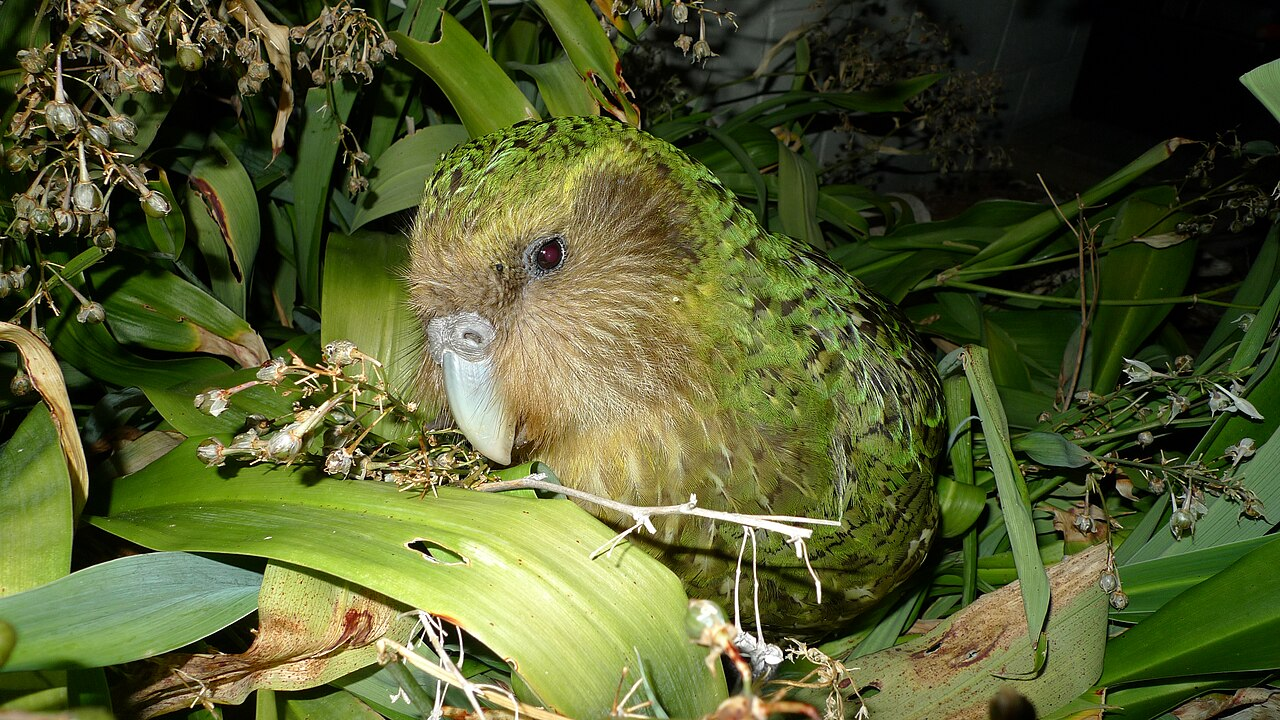
\includegraphics[width=0.46\linewidth]{images/book5/kakapo-sirocco.jpg}\hspace{0.04\linewidth}
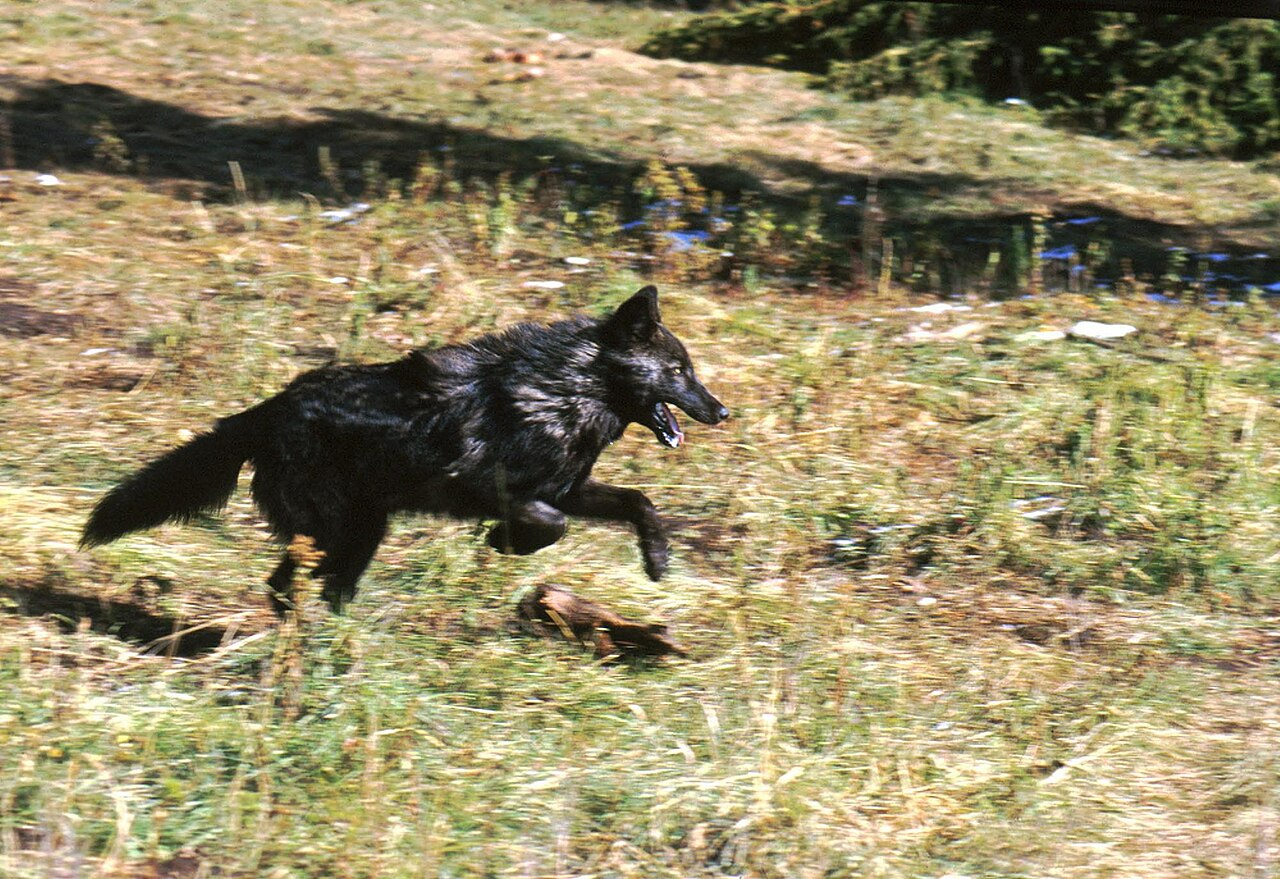
\includegraphics[width=0.46\linewidth]{images/book5/yellowstone-wolves-1996.jpg}

{\small يسارًا: سيروكو، وهو كاكابو --- أحد الناجين الواحد والخمسين عام 1995،
وأحد نحو مئتين وخمسين اليوم، كل واحد مسمّى ومراقَب على
جزر خالية من المفترسات (صورة: إدارة الصون، نيوزيلندا،
CC BY 2.0). ويمينًا: ذئاب في يلوستون عام 1996، في أول
شتاء بعد \omterm{def:b3:conservation-biology:tools}{إعادة إدخالها} (صورة: دائرة المتنزهات الوطنية،
ملكية عامة).}
\end{omfigure}

\begin{example}[ثلاثة تعافيات]\label{ex:b3:conservation-biology:recoveries}
الكاكابو: واحد وخمسون طائرًا عام 1995، نُقلت كلها إلى جزر طُهّرت من
المفترسات؛ وكل طائر يحمل مرسلًا، وكل عش يُراقَب
بكاميرا، وتُربّى الفراخ باليد حين تخفق أم، وتُطعَم الذكور
ليدخلوا في حالة التكاثر في السنوات التي تثمر فيها أشجار الريمو،
ويُدار النسب لإبقاء مورّثات آخر ذكر من فيوردلاند النادرة
في الجمهرة؛ وقد سُلسل جينوم كل كاكابو.
ومئتان وخمسون اليوم، و$N_{e}$ تضعه الجينومات قرب
مئة. والكركي الصائح: خمسة عشر طائرًا عام 1941، سربًا مهاجرًا
واحدًا، رُبّي في الأسر من بيوض أُخذت من أعشاش برية،
وعُلِّم طرق هجرة جديدة خلف طائرات خفيفة جدًا، وصار نحو ثمانمئة.
والحوت الأحدب: صِيد إلى بضعة آلاف، وحُمي في
1966، وتجاوز مئة ألف، بزيادة قرب \qty{8}{\%} في السنة
تبيّن ما يفعله حيوان طويل العمر حين يُزال السبب الوحيد
لتراجعه. وقد كلف كل تعافٍ عشرات الملايين وعقودًا؛
وحساب الفصل يقول لماذا كان لا بد أن يُبذل الجهد
قبل أن تبلغ الأعداد الدوامة، ولماذا كان أرخص من أي
إنقاذ لاحق.
\end{example}

\begin{omfigure}
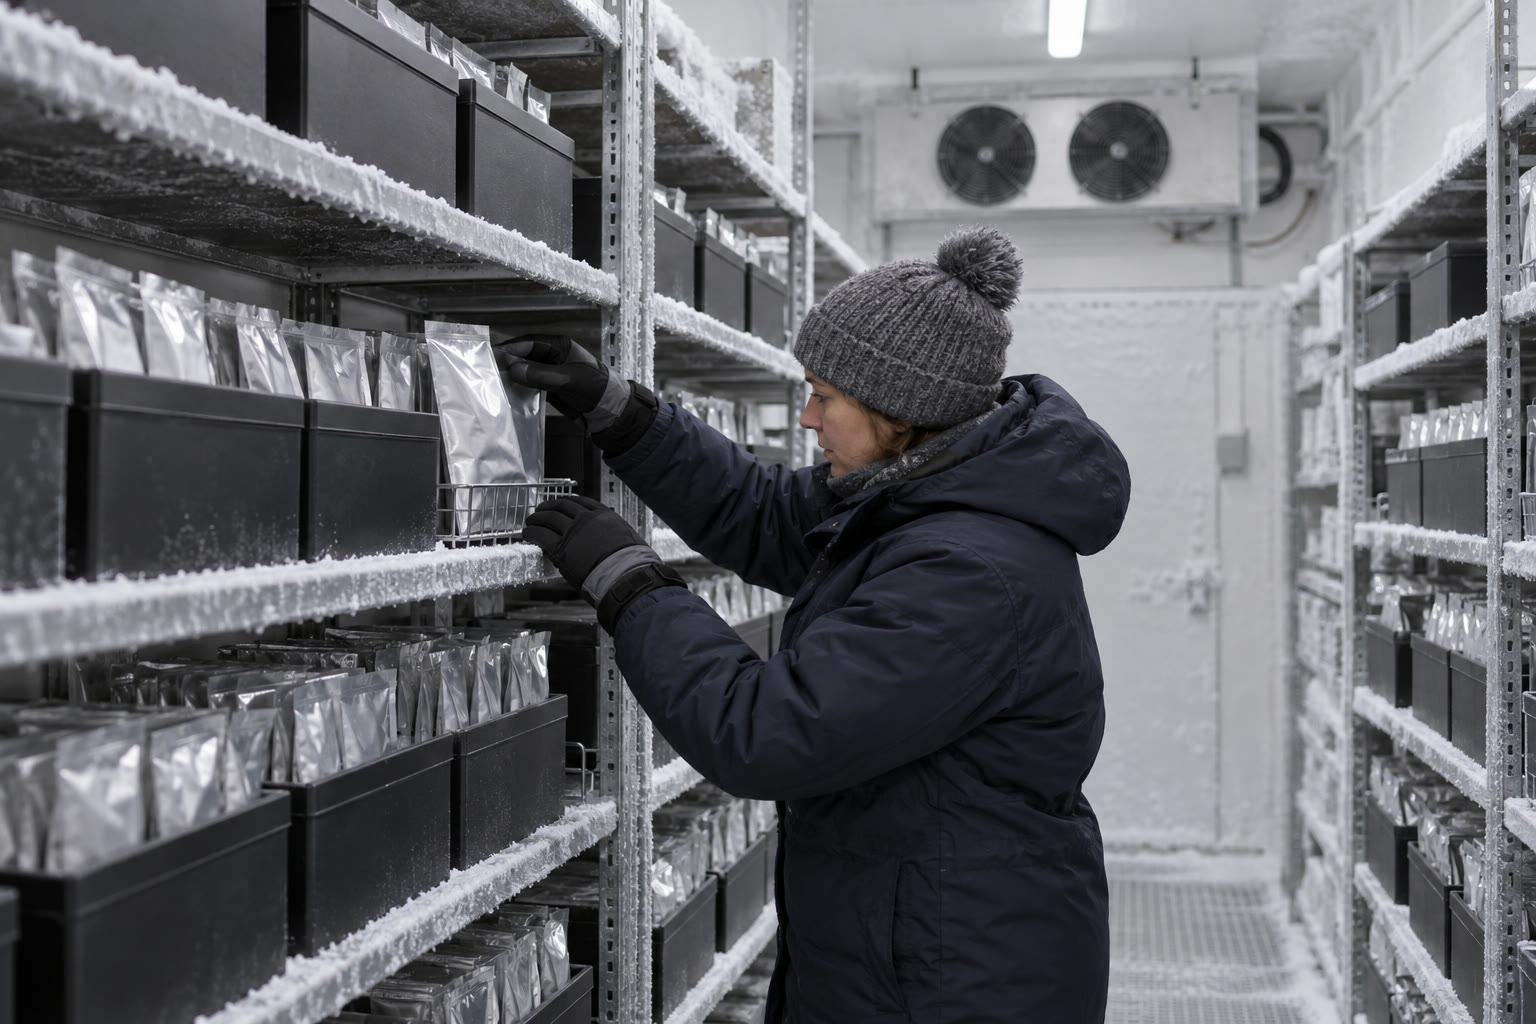
\includegraphics[width=0.56\linewidth]{images/book5/ai/b5-27-seed-vault.jpg}

{\small قبو بذور في الجليد الدائم: نسخ من مليون مدخلة من
محاصيل ونباتات برية، محفوظة عند \qty{-18}{\celsius} في مواجهة فقد
المجموعات التي جاءت منها --- أي الصون تأمينًا، على
مقياس جينوم نوع.}
\end{omfigure}

\begin{remark}[حساب الحفظ]\label{rem:b3:conservation-biology:remark}
انتهى كل فصل من هذا المنهاج بعدد، وينتهي هذا
بعدة أعداد: حجم فعال، ومعامل تزاوج داخلي يرتفع بمقدار
$1/2N_{e}$ في الجيل، وأس $z$ يحيل الهكتارات المفقودة
أنواعًا مفقودة، واحتمال انقراض على مدى قرن. وهي
خشنة --- فالتعداد غير يقيني، والتباين مخمَّن، والنموذج
كاريكاتير --- وهي ما يحيل عاطفةً نحو طيور
زائلة إلى قرار في أي خمسين هكتارًا تُشترى
وأي ثمانية حيوانات تُنقل. والبيولوجيا هي بيولوجيا سائر
الكتاب نفسها: الانجراف، والانتخاب، والديموغرافيا، والسلوك،
واعتماد الجمهرة على موئلها واعتماد الموئل على
جمهراته. والجديد هو الاستعجال وحده، وكون
التجربة تُجرى مرة واحدة، بلا شاهد، على الأنواع
الباقية.
\end{remark}

\section{تمارين}

\begin{exercise}[$\star$]\label{exo:b3:conservation-biology:1}
عرّف \omterm{def:b3:conservation-biology:small}{العشوائية الديموغرافية} \omterm{def:b3:conservation-biology:small}{والعشوائية البيئية} \omterm{def:b3:conservation-biology:small}{وأثر
ألي}، واذكر مثالًا واحدًا على كل منها من الفصل.
\end{exercise}

\begin{exercise}[$\star$]\label{exo:b3:conservation-biology:2}
ما \omterm{thm:b3:conservation-biology:ne}{الحجم الفعال للجمهرة}، وسمّ ثلاث سمات في
جمهرة حقيقية تجعله أصغر من التعداد.
\end{exercise}

\begin{exercise}[$\star$]\label{exo:b3:conservation-biology:3}
اذكر قانون الأنواع والمساحة. فإذا كان $z = 0.25$، أي نسبة من الأنواع
يبقيها موئل بعد فقد نصف مساحته؟ وتسعة أعشارها؟ وتسعة وتسعين
جزءًا من مئة؟
\end{exercise}

\begin{exercise}[$\star$]\label{exo:b3:conservation-biology:4}
اشرح قاعدة 50/500، ومِمَّ يحمي كل عدد.
\end{exercise}

\begin{exercise}[$\star\star$]\label{exo:b3:conservation-biology:5}
قطيع من 200 فقمة فيل فيه 8 ذكور متكاثرة و120 أنثى
متكاثرة. احسب $N_{e}$ وفقد \omterm{thm:b3:conservation-biology:ne}{التغايرية الزيجية} في الجيل.
وكم جيلًا حتى يُفقد ربعها؟
\end{exercise}

\begin{exercise}[$\star\star$]\label{exo:b3:conservation-biology:6}
جمهرة كانت 1000 و1000 و20 و1000 و1000 في خمسة أجيال
متعاقبة. احسب $N_{e}$ على المدى، \omterm{thm:b3:conservation-biology:ne}{والتغايرية الزيجية}
المحفوظة، وقارن ذلك بألف ثابتة.
\end{exercise}

\begin{exercise}[$\star\star$]\label{exo:b3:conservation-biology:7}
خمسة وعشرون فهدًا فلوريديًا عند $N_{e} \approx 10$: فما التزاوج
الداخلي المتراكم في 5 أجيال؟ وإذا هبطت الملاءمة \qty{5}{\%} لكل
\qty{10}{\%} من $F$، فبكم هبطت الملاءمة؟ وماذا تفعل إضافة
ثماني إناث غير قريبة في قيمة $F$ في الجيل التالي؟
\end{exercise}

\begin{exercise}[$\star\star$]\label{exo:b3:conservation-biology:8}
يلوستون: 31 ذئبًا أُطلقت في 1995--96، ونحو 100 في المتنزه بحلول
2003. قدّر $r$؛ وكم كان سيكون عددها في 2020 لو استمر النمو،
ولماذا لم يستمر؟
\end{exercise}

\begin{exercise}[$\star\star$]\label{exo:b3:conservation-biology:9}
صنّف بمعايير الاتحاد الدولي في الفصل: (أ) ضفدع هبطت
جمهرته \qty{60}{\%} في عشر سنين؛ (ب) نبات من 180 فردًا
ناضجًا؛ (ج) سمكة مداها \qty{3000}{km^2}؛ (د) طائر من
\num{30000} فرد يتراجع \qty{10}{\%} في العقد.
\end{exercise}

\begin{exercise}[$\star\star\star$]\label{exo:b3:conservation-biology:10}
جمهرة من $N$ زوج ينتج كل واحد، باحتمال $1/2$، خلفين
ناجيين وإلا فلا شيء (\omterm{def:b3:conservation-biology:small}{عشوائية ديموغرافية}).
احسب احتمال أن تخفق الجمهرة كلها في جيل
واحد عند $N = 2$ و$5$ و$10$ و$20$، وعلّق على كيف يتدرج
الخطر الديموغرافي مع $N$.
\end{exercise}

\begin{exercise}[$\star\star\star$]\label{exo:b3:conservation-biology:11}
قانون الأنواع والمساحة عند $z = 0.25$، وغابة تُقطع إلى 10 شظايا
متساوية معزولة. قارن الأنواع المتوقعة في شظية واحدة
بعُشر الأصل، واحتجّ لماذا لا يكون المجموع عبر الشظايا
هو الأصل بالبساطة --- وما الذي يحدد هل تحوي الشظايا
معًا أنواعًا أكثر أم أقل مما حواه الكل؟
\end{exercise}

\begin{exercise}[$\star\star\star$]\label{exo:b3:conservation-biology:12}
لماذا توقف إضافةُ بضعة مهاجرين في الجيل ($m N_{e} \approx 1$)
فقدَ التباين في جمهرة صغيرة في معظمه، وماذا يكلف ذلك
في التأقلم الموضعي؟ استعمل الميزان بين الانجراف، $1/2N_{e}$،
ونسبة الأليلات التي يستبدلها المهاجرون، $m$، في الحجة.
\end{exercise}

\section{مسألة: خمسون وخمسمئة}

\begin{problem}[{مسألة نهاية الأسبوع --- برنامج تعافٍ بالأرقام:
الحجم الفعال لجمهرة ببغاء مُنقَذة وتزاوجها الداخلي، وإنقاذ
وراثي، والأنواع التي ستبقيها غابة متقلّصة، ونمو
ذئاب معادة الإدخال، والخانات والكلف، وتُختم بقيمة $N_{e}$،
وبالتزاوج الداخلي بعد عشرة أجيال، وبنسبة الأنواع المحفوظة}]
\label{pb:b3:conservation-biology:1}
المعطيات: جمهرة ببغاء من 60 بالغًا، 20 ذكرًا و40 أنثى، كلها
متكاثرة؛ وزمن الجيل \qty{10}{yr}. وتاريخ الجمهرة في الأجيال
الخمسة الأخيرة: 500 و100 و60 و51 و60. وتدهور التزاوج الداخلي:
تهبط الملاءمة \qty{6}{\%} لكل \qty{0.1}{} من $F$. والإنقاذ: 10
طيور غير قريبة تُضاف إلى 60. والغابة: \qty{2000}{km^2} تُخفَّض إلى
\qty{300}{km^2}، و$z = 0.25$؛ والأنواع الآن 180. والذئاب: 31 أُطلقت، و100
بعد 8 سنين، والسعة الحملية في المتنزه نحو 120. والكلفة: أربعة
ملايين دولار في السنة للببغاوات.

\medskip
\noindent\textbf{الجزء الأول --- الحجم الفعال.}
\begin{enumerate}
  \item $N_{e}$ من \omterm{thm:b3:conservation-biology:ne}{نسبة الجنسين} في الستين الحالية. قارنه
        بالتعداد.
  \item $N_{e}$ \omterm{thm:b3:conservation-biology:ne}{بالوسط التوافقي} على أجيال التاريخ الخمسة.
        وأي جيل يهيمن؟
  \item التزاوج الداخلي المتراكم على تلك الأجيال الخمسة،
        باستعمال $N_{e}$ \omterm{thm:b3:conservation-biology:ne}{الوسط التوافقي} (بالصيغة التامة وبالتقريب الخطي).
  \item الملاءمة المفقودة بذلك التزاوج الداخلي.
  \item \omterm{thm:b3:conservation-biology:ne}{التغايرية الزيجية} المحفوظة بعد الأجيال الخمسة، كنسبة
        من الأصل.
  \item إذا أُبقيت الجمهرة الآن عند 60 \omterm{thm:b3:conservation-biology:ne}{بنسبة الجنسين}
        الحالية، فأي $F$ ستبلغ في عشرة أجيال أخرى، وأي
        فقد للملاءمة؟ وكم سنة ذلك؟
\end{enumerate}

\medskip
\noindent\textbf{الجزء الثاني --- الإنقاذ.}
\begin{enumerate}[resume]
  \item عشرة طيور غير قريبة تنضم إلى الستين. ونسبة الأليلات في
        الجيل التالي الآتية من الوافدين نحو $10/70$؛ \omterm{thm:b3:conservation-biology:ne}{ومعامل
        التزاوج الداخلي} لخلف أحد والديه أصلي والآخر وافد
        $0$. قدّر متوسط $F$ في الجمهرة في
        الجيل التالي إذا كان التزاوج عشوائيًا.
  \item اشرح لماذا يهبط $F$ فورًا وترتفع \omterm{thm:b3:conservation-biology:ne}{التغايرية الزيجية}
        فقط مع انتشار أليلات المهاجرين، ولماذا قد يلزم
        إنقاذ ثانٍ.
  \item لبلوغ $N_{e} = 500$ بنسبة جنسين متساوية، كم بالغًا
        يلزم؟ وعند $r = \qty{0.05}{yr^{-1}}$ من 70 طائرًا، كم
        سنة؟
  \item يزيل البرنامج البيوض من الأمهات الرديئات للتربية
        باليد، فيرفع متوسط عدد الفراخ المُريَّشة لكل زوج لكنه يساوي
        بين أحجام الأسر. فلماذا \emph{يرفع} تساوي أحجام الأسر
        $N_{e}$ فوق التعداد (نحو $2N$)؟
  \item آخر ذكر من سلالة جنوبية متميزة عقيم في
        البرية. اقترح تدخلين وكلفتيهما على مجمع
        المورّثات.
  \item عند أربعة ملايين دولار في السنة على مدى 40 سنة لبلوغ
        $N_{e} = 500$، ما الكلفة الكلية، والكلفة لكل طائر مضاف؟ وهل ذلك غالٍ؟ وفي مقابل
        ماذا؟
\end{enumerate}

\medskip
\noindent\textbf{الجزء الثالث --- الغابة.}
\begin{enumerate}[resume]
  \item نسبة الأنواع التي ستبقيها الغابة عند \qty{300}{km^2}؛
        والعدد المتوقع للأنواع، ودين الانقراض (الأنواع
        الحاضرة الآن التي ستُفقد).
  \item ولو كانت \qty{300}{km^2} ثلاث شظايا معزولة من
        \qty{100}{km^2}، فكم نوعًا في كل شظية؛ والمجموع لو حوت الشظايا
        أنواعًا مختلفة تمامًا؛ والمجموع لو كانت متطابقة. وما
        الذي يقرر؟
  \item ممر من \qty{20}{km^2} يصل الشظايا الثلاث. عاملها
        مساحةً واحدة من \qty{320}{km^2}: فكم نوعًا يُتوقَّع؟ قارن
        ذلك بحالة الأنواع المتطابقة في السؤال~14.
  \item أكبر مفترس في الغابة يحتاج إلى \qty{50}{km^2} لكل زوج
        وإلى $N_{e}$ قدره 50 ليدوم. فهل تقدر \qty{300}{km^2} كلها على
        حمله؟ وهل تقدر شظية؟ وبماذا يدل ذلك على المساحة في مقابل عدد
        الأنواع معيارًا؟
  \item قدّر كم يستغرق تسديد دين الانقراض إذا كانت
        الأنواع المفقودة جمهراتها تتراجع \qty{3}{\%} في السنة
        من 200 إلى عتبة \omterm{met:b3:conservation-biology:pva}{شبه انقراض} قدرها 10.
  \item لماذا يقلّل قانون الأنواع والمساحة من تقدير الفقد حين
        يضيف التفتيت آثار حافة، ويبالغ فيه حين تكون
        الأرض المحيطة قابلة للاستعمال جزئيًا؟
\end{enumerate}

\medskip
\noindent\textbf{الجزء الرابع --- الذئاب والقوائم.}
\begin{enumerate}[resume]
  \item الذئاب: $r$ من $31 \to 100$ في 8 سنين، وزمن المضاعفة.
  \item نمو لوجستي نحو $K = 120$: الجمهرة بعد 8 سنين
        تحت نمو لوجستي لا أسّي، ابتداءً من 31
        بالمقدار $r$ في السؤال~19 (استعمل $N(t) = K/[1 + (K/N_{0} -
        1)\mathrm{e}^{-rt}]$). فأيهما يطابق المرصود 100 أفضل، وبماذا
        يدل ذلك على الاعتماد على الكثافة في السنين الأولى؟
  \item كانت الأيائل \num{17000} عام 1995 و\num{4000} عام 2015.
        فما متوسط معدل التراجع السنوي؟ وكم منه تفسره ذئاب تأكل
        \num{20} أيلًا كل واحدة في السنة عند 100 ذئب؟
  \item صنّف الببغاء (60 فردًا ناضجًا) ومفترس الغابة قبل
        الإنقاذ بمعايير الاتحاد الدولي.
  \item الحمام الزاجر: خمسة مليارات عام 1800، ومنقرض عام 1914. فإذا كان
        التراجع أسّيًا من 1870، حين كانت لا تزال بالمليارات،
        إلى طائر واحد عام 1914، فأي معدل سنوي يقتضي ذلك؟
        ولماذا يجعل \omterm{def:b3:conservation-biology:small}{أثر ألي} العقود الأخيرة أسرع من الأسّي؟
  \item اشرح في فقرة لماذا كان تحليل قابلية البقاء سيقول إن الحمام
        الزاجر آمن عام 1850، وما الذي كان سيفوته.
  \item لخّص: قيمة $N_{e}$ الحالية (السؤال~1)، و$F$ بعد عشرة
        أجيال أخرى عند 60 (السؤال~6)، ونسبة الأنواع التي تبقيها
        الغابة المتقلّصة (السؤال~13).
\end{enumerate}
\end{problem}
